\documentclass[10pt]{article}

\usepackage[margin=1.5in]{geometry}
\usepackage{graphicx}
\usepackage{natbib}
%correct punctuation for MBE
\bibpunct[,]{(}{)}{;}{a}{}{,}
\usepackage{tablefootnote}
\usepackage{amsmath}

\renewcommand{\bottomfraction}{.9}
\renewcommand{\topfraction}{.9}
\renewcommand{\textfraction}{0.1}
\renewcommand{\floatpagefraction}{.9}

\linespread{1.5}
\begin{document}

\title{\textbf{Masking individual residues in alignments for positive-selection inference has limited utility}}
\author{Stephanie J. Spielman$^{1*}$ and Eric T. Dawson$^{1}$ Claus O. Wilke$^{1}$}
\date{}

\maketitle
\noindent
Address:\\
$^1$Section of Integrative Biology and Center for Computational Biology and Bioinformatics. The University
of Texas at Austin, Austin, TX 78731, USA.\\

\bigskip
\noindent
$^*$Corresponding author\\
$\phantom{^*}$Email: stephanie.spielman@utexas.edu\\

\bigskip
\noindent
Manuscript type: research article

\bigskip
\noindent Keywords: multiple sequence alignment, alignment filters, positive-selection inference, sequence simulation

\newpage
\begin{abstract}
 Recent studies have noted that errors in multiple sequence alignments have the potential to reduce accuracy in positive-selection inference. Many have therefore suggested that users filter their alignments before further analyses. One widely-used filter, known as Guidance, generates position-based confidence scores for a given alignment using a bootstrap approach, thereby allowing users to remove positions of low confidence from the alignment. However, the specific circumstances under which Guidance offers improvements has been unclear. To elucidate how the Guidance filter behaved in realistic protein-coding sequences, we have reimplemented the Guidance software to include two novel algorithms for phylogenetically correcting confidence scores. We additionally introduced a new score normalization scheme which assigned lower scores to highly-gapped alignment columns. Using a sequence simulation approach, we compared our reimplemented Guidance algorithms to the original and found, surprisingly, that no approach examined could substantially improve positive-selection inference. Thus, we cannot equivocally advocate the use of a Guidance-based filter for such studies.
\end{abstract}


\section*{Introduction}
Constructing a multiple sequence alignment represents the first step of analysis in most studies of molecular evolution, namely phylogenetic reconstruction and evolutionary rate inference. Recently, several studies have shown that poor alignment quality can significantly hinder accuracy in such downstream analyses \citep{Jordan2011, MarkovaRaina2011, Dwivedi2009, Talavera2007, Ogden2006}. In particular, using low-quality MSAs during positive-selection inference elevated false positive rates \citep{Privman2012, Schneider2009, Fletcher2010}. As a consequence, many have advocated applying an alignment filter to MSAs. Such filters, which include Guidance \citep{Penn2010, Privman2012}, GBLOCKS \citep{Castresana2000} and T-Coffee \citep{Notredame2000}, locate putatively poorly aligned regions in alignments, thereby allowing users to curate their alignments to maximize signal. The hope is that culling unreliable positions and/or columns from MSAs will yield increased accuracy in positive-selection inference, without excessively sacrificing power.

Of these filters, Guidance \citep{Penn2010} is currently the most widely used in positive-selection inference. Guidance derives a confidence score for each MSA position using a bootstrap approach that samples variants in a progressive alignment guide tree. Using the resulting scores, users can mask (i.e. replace with an ambiguous character such as ``?" or ``N") positions which score below a given threshold, thereby removing residues that cannot be confidently placed in the alignment. This method is fairly conservative, as particular positions of low confidence can be removed rather than entire columns. Recent simulation studies have demonstrated that filtering poorly aligned residues with Guidance may increase accuracy when inferring positive selection \citep{Jordan2011,Privman2012}. 

However, while Privman et al. \citet{Privman2012} found dramatic improvements in positive-selection inference when applying the Guidance filter, Jordan and Goldman's \citet{Jordan2011} comprehensive study on alignment methods and filtering found that Guidance modestly, if at all, affected this inference. In particular, they reported that, at lower protein divergence levels or insertion/deletion (indel) rates, Guidance neither substantially improved nor worsened positive selection detection. Alternatively, at high divergence levels (1.8 mean path length, defined as mean root-to-tip branch length) or indel rates (0.2 indel/substitution events), Jordan and Goldman found that Guidance significantly boosted true positive rates. While these results were compelling, protein sequences used in positive selection studies rarely, if ever, contain sequences separated by such high divergences; for example, a typical mammalian gene tree's MPL is only about 0.17 \citep{Spielman2013}, 10\% the divergence level at which Jordan and Goldman detected improvements when using the Guidance filter.

Motivated by these apparent discrepancies, we sought to determine whether altering the Guidance scoring algorithm could improve positive-selection inference at more realistic divergences. To this end, we reimplemented the Guidance software (see Methods for details) and examined the effects of new scoring algorithms which take the sequences' phylogenetic relationships into account. Using this reimplementation, we filtered alignments produced from realistic protein-coding sequence simulations and subsequently inferred positive selection with two methods: the recently-described method Fubar \citep{Murrell2013} and the current standard of use, Paml's M8 model \citep{Yang2007}. Overall, we found that neither the original Guidance filter nor our newly implemented filters conferred any substantial changes to positive-selection inference, and any benefits recovered were of extremely small magnitude. Thus, we cannot unequivocally advocate the use of such filters when inferring positive selection in protein-coding sequences.


\section*{Results}

\subsection*{Guidance reimplementation and analysis pipeline}
To systematically evaluate Guidance's influence on positive-selection inference, we reimplemented the Guidance software in python and C++. Before conducting any analyses, we verified that, given a set of perturbed alignments, our program produced the same confidence scores as the original Guidance. In addition to our basic Guidance reimplementation, we derived two new algorithms which employ phylogenetic weighting when assigning confidence scores (see Methods for details).  Briefly, the first method incorporated a weight for each sequence in the alignment, as calculated by BranchManager \citep{Stone2007}, and the second method incorporated patristic distances (the sum of branch lengths between two taxa). We called these methods, respectively, BMweights and PDweights.  We additionally proposed a ``gap-penalization" score normalization scheme, which naturally assigned lower confidence scores to residues in highly gapped regions, given that such regions were more likely to be poorly aligned. We referred to filters using the gap-penalization scheme as GuidanceP, BMweightsP, and PDweightsP.

We began by simulating 100 realistic protein-coding sequences using Indelible \citep{Fletcher2009} along each of four different gene trees sizes 11, 26, 60, and 158 taxa. To ensure that these simulations produced real sequence data to the extent possible, we simulated according to evolutionary parameters inferred from H1N1 influenza hemagluttinin (HA), a protein well known to contain positively selected regions \citep{Meyer2012}. We then processed the unaligned sequences with our Guidance reimplementation using the aligner mafft L-INS-I (linsi) \citep{Katoh2005}. We chose to use only linsi, which strongly outperforms other similar alignment softwares for protein alignments \citep{Thompson2011,Nuin2006} without sacrificing speed. We scored each alignment using each of our three scoring algorithms (original Guidance, BMweights, and PDweights) with each of our two normalization schemes (original Guidance and gap-penalization), and masked positions with scores below 0.5 with ``?".

Finally, we assessed positive selection with both the recently-described Fubar \citep{Murrell2013} as implemented in HyPhy \citep{Pond2005} and the widely-used M8 model in Paml \citep{Yang2007}. Note that we use Paml throughout this paper to refer specifically to the M8 model.  All phylogenies used during these inferences were constructed on from unfiltered amino acid alignments in RAxML \citep{Stamatakis2006} using the CAT model under the WAG substitution matrix. All filtered alignments stemming from the same unfiltered alignment were analyzed with the same phylogeny to remove any potential bias that distinct phylogenies could introduce.We considered sites as positively selected if the given method returned a posterior probability $\geq0.90$. Note that, while we processed all alignments with Fubar, we did not infer positive selection for the largest simulation set with Paml due to prohibitive runtimes. 


\subsection*{Filtering with Guidance-based methods has a minimal effect}

We assessed how filtering alignments with a Guidance-based method influences positive selection detection by comparing the resulting true positive rates (TPRs) of positive-selection inference between all filtered alignments and their corresponding unfiltered alignments. To this end, we build mixed-effects linear models for each sequence simulation set, with simulation count as the random effect to account for the paired structure of our analysis (as in, each alignment was filtered with multiple strategies, rendering them dependent), for Fubar and Paml separately. We chose to primarily compare the TPRs among alignments as opposed to the false positive rates (FPRs), as FPRs were exceedingly small, never exceeding an average of 0.017 across simulation sets and methods. These rates were similar to those recovered by \citep{Jordan2011}. 

We first compared the two normalization schemes, original and gap-penalization, to one another using mixed effects models with TPR as the response variable, simulation count as a random effect, and normalization scheme as a fixed effect. Only filtered alignments were considered in these models, results from which are seen in Table \ref{tab:penalmodel}. In all instances in which we detected significant difference between normalization schemes, the gap-penalization scheme outperformed the original Guidance scheme, albeit by very small magnitudes. Therefore, we proceeded to compare the results from gap-penalization algorithms (GuidanceP, BMweightsP, PDweightsP) to those of unfiltered alignments with a second series of mixed-effects models. These models included TPR as the response variable, simulation count as a random effect, and algorithm as a fixed effect. Table \ref{tab:casemodel} gives the results from these models for each simulation set and selection inference method.

Overall, we did not recover any difference in TPR among gap-penalization filtering algorithms; Guidance and the two phylogenetically-weighted methods performed statistically indistinguishably for a given simulation set. Figure \ref{roc} displays ROC curves for positive-selection inference with Fubar and Paml. Figure \ref{roc}B highlights the effect of alignment filtering with Fubar and Figure \ref{roc}C with Paml; for each method, respectively, areas under the unfiltered alignment curves were essentially the same as for the filtered alignment curves.

When processed with Fubar, alignment filtering significantly increased TPRs for the 60 and 158-sequence simulation sets. The magnitude of its improvements were very small, boosting unfiltered TPRs by an average of 0.03 for the 60-sequence set and by 0.01 for the 158-sequence set. In other words, TPR increased by 10\% for the 60-sequence simulation set and by 3\% for the 158-sequence simulation set. Filtering neither improved nor worsened positive-selection inference for the 11 or 26-sequence simulation sets as analyzed with Fubar.

Analyzing the data with Paml similarly did not result in a significant TPR change for the 11-sequence simulation set. Unlike when analyzing with Fubar, we did not recover significant TPR changes for the 60-sequence simulation set. Alternatively, Paml results showed that filtering did improve TPRs in the 26-sequence simulation set, albeit by an average of roughly 0.009. While statistically significant, an increase of this low a magnitude may not have any noticeable effect on positive-selection inference in studies of real sequences. 

\subsection*{Influence of Posterior Probability on Selection Inference Methods}

Our analysis recovered several differences in how Paml and Fubar behaved when assessing positive selection. In particular, whether Fubar or Paml performed better depended on the number of sequences analyzed; Fubar outperformed Paml for the two smaller simulation sets of 11 and 26-sequences, but Paml outperformed Fubar for the 60-sequence simulation set (Table \ref{tab:casemodel}). We found that this trend resulted from the posterior probability threshold chosen to call sites as positively selected. Figure \ref{tprfpr}shows how TPRs and FPRs for unfiltered alignments behaved for two different simulation sets (26 and 60-sequence) across posterior probability cutoffs. With regards to TPRs,
Fubar generally performed better than Paml at lower posterior probabilities, whereas Paml outperformed Fubar at high probabilities. As the number of sequences increased, the intersection between methods' TPRs shifted towards lower posterior probabilities. Paml's improved ability to call true positives with the inclusion of more sequences largely dictated this shift, as Fubar's relationship between posterior probability and TPR remained similar between the two simulation sets.  Filtering alignments only marginally, if at all, affected these broad trends that Fubar and Paml portrayed, as seen in Figure \ref{fulltpr}). Thus, the analysis method used affected positive-selection inference substantially more than did filtering  alignments with a Guidance-based method. \textbf{possible statement about how it's ok our model was at 0.9. Don't think necessary, though}.

The relationship between posterior probability and FPR, unlike that of TPR, was mostly consistent across simulation sets for both Fubar and Paml. While Paml achieved FPRs of nearly zero essentially immediately for both the 26 and 60-sequence simulation sets, Fubar approached a zero FPR more slowly, reaching zero around a posterior probability of 0.8 for each simulation set. As a typical study of positive selection would almost definitely use a posterior probability above at least 0.8, alignment filtering would likely not be able to substantially reduce FPR.

How TPR and FPR behaved for Fubar and Paml evidenced the different approaches these methods employ to detect positive selection; while Paml's M8 model aims to identify precise $dN/dS$ value at each site in an alignment, Fubar merely approximates whether a site is positively selected but does not attempt to assign a point estimate of $dN/dS$ to each position. With fewer sequences in an alignment, then, Paml was less accurate at determining  a particular site's exact $dN/dS$ would be less precise than was Fubar at simply approximating whether that position was positively selected. Increasing the number of sequences allowed for Paml to make more robust $dN/dS$ estimates while having a relatively smaller effect on Fubar's approximations.

%%%%%%%%%%%%%%%%%%%     OLD TEXT WE MAY WANT TO KEEP AROUND IN CASE %%%%%%%%%%%%%%%%%%%
%ROC curves did not control for the posterior probability threshold employed to call sites as positively selected. In other words, a given point on an ROC curve could easily correspond to different posterior probability thresholds for filtered and unfiltered alignments. Thus, while useful in assessing theoretical performance, ROC curves did not capture the reality of data analysis and might actually have been misleading.
%%%%%%%%%%%%%%%%%%%%%%%%%%%%%%%%%%%%%%%%%%%%%%%%%%%%%%%%%%%%%%%%%%%%%%










\section*{Discussion}

We have conducted a simulation-based study to evaluate the how introducing phylogenetically-aware scoring algorithms into the Guidance alignment filter influences the detection of positive selection in protein-coding sequences. Additionally, we tested a novel method for normalizing Guidance scores, using both the original Guidance algorithm and our phylogenetically-corrected methods, which assigns inherently lower scores to highly-gapped columns in an alignment. We ensured that our simulations resembled real sequence data by simulating along real gene trees according to evolutionary parameters derived from the H1N1 influenza hemagluttinin protein. We inferred positive selection for all alignments using two methods: the recently introduced and very fast Fubar \citep{Murrell2013} within the HyPhy package \citep{Pond2005} as well as the current standard for evolutionary rate inference, Paml \citep{Yang2007} (specifically the M8 model).

We found that, while the gap-penalization scheme marginally improved upon the original normalization method, incorporating phylogenetic information into the scoring scheme did not significantly change accuracy in such analyses. Even so, filtering alignments with any Guidance-based method, including the original, did not substantially improve positive-selection inference under any circumstance. That the phylogenetically-weighted algorithms did not improve upon the original Guidance algorithm indicated the minimal benefits that filtering in this manner produced at all. Were the original Guidance to offer robust improvements in positive selection detection, one might expect that our more statistically controlled approach would boost the method's performance. However, as we have found that masking individual positions in an alignment only marginally affected positive-selection inference in the first place, one might not expect the algorithmic changes we implemented might to have a dramatic effect.

While others have noted a prevalence of false positives in positive-selection inference, we recovered very low false positive rates. The FPRs we detected were very similar to those of Jordan and Goldman \citet{Jordan2011}, yet substantially lower than those detected by Privman et al. \citet{Privman2012}. \textbf{I am very scared to comment on the Guidance paper at all because I don't think I can do it without it seeming like an attack. Any advice here?} We attributed our small FPRs to the fact that we employed simulated sequences, which represents the only strategy to assess methodological accuracy with complete confidence. While though we took strong measures to ensure that our simulated sequences resembled real data to the extent possible, it is impossible for simulated data to fully capture the evolutionary process. Even so, our realistic simulations did indicate that, while alignment filtering offered some benefits, those improvements were marginal, at best. Indeed, with such minimal changes to positive-selection inference, alignment filtering could easily decrease accuracy in a given positive selection study.  

Overall, we cannot unequivocally recommend the use of a Guidance-based alignment filter when inferring evolutionary rates. Once an alignment has been constructed, it does not seem that much can be done to eliminate any misleading information. Instead, researchers should select inference methods in which the error can be minimized as much as possible without necessitating post-hoc correction. Therefore, we recommend that users select high-quality alignment and positive-selection inference methods to minimize any obscuring signal rather than relying on filters.


\section*{Methods}

\subsection*{Guidance Reimplementation}
Our reimplemented Guidance is written in Python and C++. Following the algorithm set forth in Penn et al. \citep{Penn2010}, we first create a reference amino-acid alignment using a user-specified progressive alignment software, with choices of clustalw \citep{Thompson1994}, muscle \citep{Edgar2004}, or mafft \citep{Katoh2002, Katoh2005}. We then generate 100 bootstrapped alignment replicates, each of which is used to create a bootstrapped tree in FastTree2 \citep{Price2010}. We then use these 100 trees as guide trees to create 100 new perturbed alignments, which we subsequently compared to the reference alignment to generate a confidence score for each residue.

\subsection*{Scoring Algorithms}
As additionally implemented two new scoring algorithms which incorporating phylogenetic information. Before calculating scores, a phylogeny is built from the reference alignment. Our program includes functionality to build this phylogeny using either either FastTree2 \citep{Price2010} or RAxML \citep{Stamatakis2006}. Using this phylogeny, two types of phylogenetic weights can be calculated. The first uses the software package BranchManager \citep{Stone2007} to calculate a weight for each taxon in the phylogeny representing that taxon's contribution to the phylogeny as a whole. We call this method ``BMweights." The second method calculates patristic distances (sum of branch lengths) between each taxon in the phylogeny using the python package DendroPy \citep{Sukumaran2010}. We call this method ``PDweights."

We calculated positional confidence scores for each of the $n$ bootstrap alignment as follows. A raw score, $S$, for a given residue in row $i$, column $j$ of the reference alignment is calculated as \begin{equation} S_{ij} = \sum\limits_{}^k I_{ik}^j s_{ik}^j \end{equation}, where $k$ represents all rows in column $j$ which are not gaps. 
In this formula, the indicator function 
\begin{equation}I_{ik}^j = \left\{ \begin{array}{rl}

              1                         &\mbox{if reference alignment residue pair (i,k) is present in bootstrap alignment} \\
              0            &\mbox{if reference alignment residue pair (i,k) is absent in bootstrap alignment} \\
                     \end{array} \right. 
\end{equation}
served to compare the bootstrap and reference alignment residue pairings.
We calculated $s_{ik}^j$ based on the given scoring algorithm:

\begin{equation}
s_{ik}^j = \left\{ \begin{array}{rl}

              1                         &\mbox{if Guidance} \\
              w_iw_k              &\mbox{if BMweights} \\
              d_p(i,k)              &\mbox{if PDweights} \\
                     \end{array} \right.,
\end{equation}

where $w_i$ was the phylogenetic weight of the taxon at row $i$, as calculated by BranchManager, and $d_p(k,i)$ was the patristic distance between the taxa at rows $i$ and $k$. 

We then summed positional scores $S_{ij}$ determined from each bootstrap alignment and normalized them to yield a final score $\widetilde{S}_{ij}$ at each residue in the reference alignment. We used two different normalization schemes to this end. The first scheme, given by \begin{equation} \widetilde{S}_{ij} = \frac{\sum\limits_{}^n S_{ij}}{n\sum\limits_{}^k S_{kj}}, \end{equation} normalized by only considering the residue-residue comparisons made, as done by \citep{Penn2010}. The second scheme was given by 

\begin{equation} \widetilde{S}_{ij} = (\sum\limits_{}^n S_{ij}) \bigg/ \left\{ \begin{array}{rl}
              n\times (l-1)                                   &\mbox{if Guidance} \\
              n\sum d_p(i,l)                         &\mbox{if BMweights} \\
   		  nw_i                                       &\mbox{if PDweights} \\          
         \end{array} \right.,
\end{equation}
where $l$ represented all rows (including gaps) in column $j$ \textbf{l is used in two diff ways in the above formula -- the ``if Guidance" one is a number and the ``if BMweights" one is a counter. Thoughts?}. This second normalization scheme inherently gave lower scores to highly gapped columns, and we therefore called it the ``gap-penalization" normalization. We refer to the algorithms normalized by the first scheme as Guidance, BMweights, and PDweights. When normalized with the gap-penalization scheme, we refer to them, respectively, as GuidanceP, BMweightsP, and PDweightsP.



\subsection*{Sequence Simulation}
Coding sequences were simulated using Indelible \citep{Fletcher2009}. To ensure that our simulations reflected realistic protein sequences, we simulated according to evolutionary parameters of the H1N1 hemagluttinin (HA) influenza protein. To derive these parameters, we aligned 1028 HA protein sequences with mafft linsi \citep{Katoh2005} and then back-translated to a codon alignment using the original nucleotide sequence data. We generated a phylogeny from this codon alignment in RAxML \citep{Stamatakis2006} using the GTRGAMMA model. Using the codon alignment and phylogeny, we inferred evolutionary parameters with the REL (random effects likelihood)  method \citep{NielsenYang1998} using the software HyPhy \citep{Pond2005}, with five evolutionary rate categories as free parameters under the GY94 evolutionary model \citep{GoldmanYang1994}. We employed a Bayes Empirical Bayes approach \citep{Yang2000} to obtain infer $dN/dS$ values at each site, which we used to assess a complete distribution of site rates. The resulting distribution was log-normal with a mean $dN/dS = 0.37$ with 8.3\% of sites  under positive selection ($dN/dS>1$). We binned these rates into 50 equally spaced categories for specification in Indelible, which required a discrete distribution of $dN/dS$ values. Again according to parameters derived from the HA analysis, we fixed kappa ($\kappa = TI/TV$) 5.3 for all simulations. We additionally set the state codon frequencies for our simulations according to those directly calculated from HA alignment. 

We simulated 100 alignments across four different real gene trees each, yielding a total of 400 simulated alignments. Phylogenies used included an 11-taxon tree of the mammalian olfactory receptor OR5AP2 \citep{Spielman2013}, a 26-taxon tree of mammalian rhodopsin sequences \citep{Spielman2013}, a 60-sequence tree of phosphoribulokinase (PRK) genes from photosynthetic eukaryotes \citep{Yang2011}, and a 158-taxon multilocus tree of flatfish sequences \citep{Betancur2013}. The latter two phylogenies were obtained from TreeBase.
For each simulation set, we directly calculated an indel (insertion-deletion) rates directly from these trees’ original alignments, to use as simulation parameters, by dividing the total number of gaps present by the total number of positions in each alignment. Respectively, indel rates were 0.053, 0.019, 0.0041, and 0.0066. 

\subsection*{Alignment and Positive Selection Inference}
We constructed all alignments mafft linsi \citep{Katoh2002,Katoh2005} within the context of our Guidance reimplementation. In addition to an unfiltered alignment, we generated six filtered alignments (one for each filtering algorithm and each normalization scheme), masking residues with scores below cutoff of 0.5. We inferred positive selection for every condition using both Fubar \citep{Murrell2013} with default parameters and the Paml's M8 model, specifying $F3\times4$ codon frequency and ``cleandata = 0" in the control file \citep{Yang2007}. We used the phylogeny built during the Guidance alignment procedure as the input phylogeny for selection inference such that all alignments derived from the same unfiltered alignment were processed with identical phylogenies. Note that while we employed Fubar to assess positive selection for all simulation sets, we did not use Paml to infer positive selection for the largest set (158 sequences).

We then compared resulting positive-selection inferences for each alignment to its respective true alignment's $dN/dS$ values, given by Indelible during simulation, to assess performance accuracy. As residues may be differently aligned relative to the true simulated alignment, we adopted a consensus method to compare alignments we constructed to the true simulations. We required that at least 50\% of the residues present in a true alignment column be present in an inferred alignment column. If this condition was met, we considered the true alignment column’s $dN/dS$  selection status (negative, neutral, or positive) to be the true value for the given inferred column. We considered sites positively selected if the posterior probability of $(dN/dS>1) \geq 0.9$.

Statistics were performed using in-house python and R scripts. Linear modeling was conducted using the R packages lme4 \citep{Bates2012} and
multcomp \citep{Hothorn2008}. All code used is available at \textbf{the github or something}.



\begin{figure*}[H]
\centerline{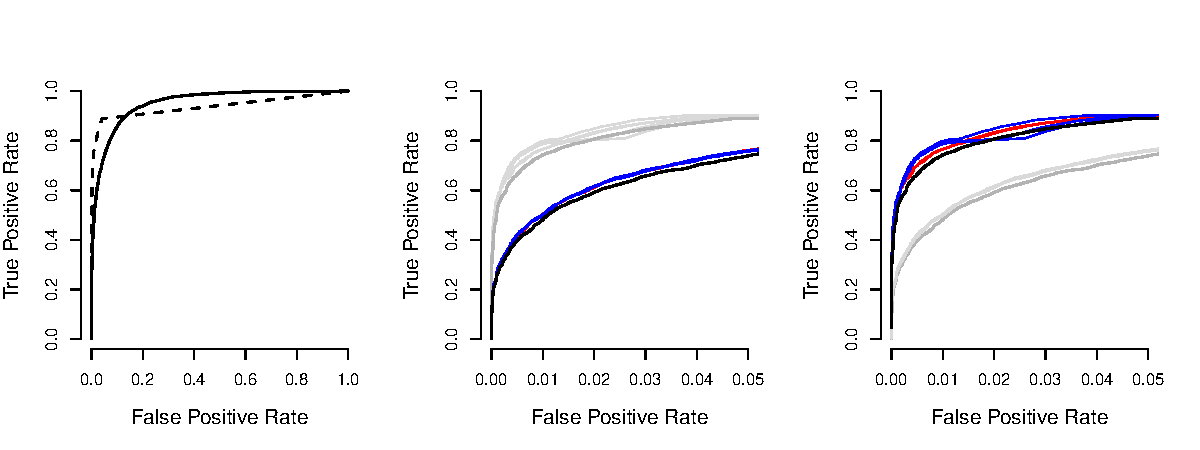
\includegraphics[width=7in]{Figures/roc.pdf}}
\caption{\label{roc} ROC curve as averaged across 60-sequence simulation set. A) Unfiltered alignments for Fubar (solid) and Paml (dashed). Note that neither method achieved FPRs greater than shown. B) Fubar in color with Paml results shown in grey. C) Paml in color with Fubar results shown in grey.}
\end{figure*}



\begin{figure*}[H]
\label{tprfpr}
\centerline{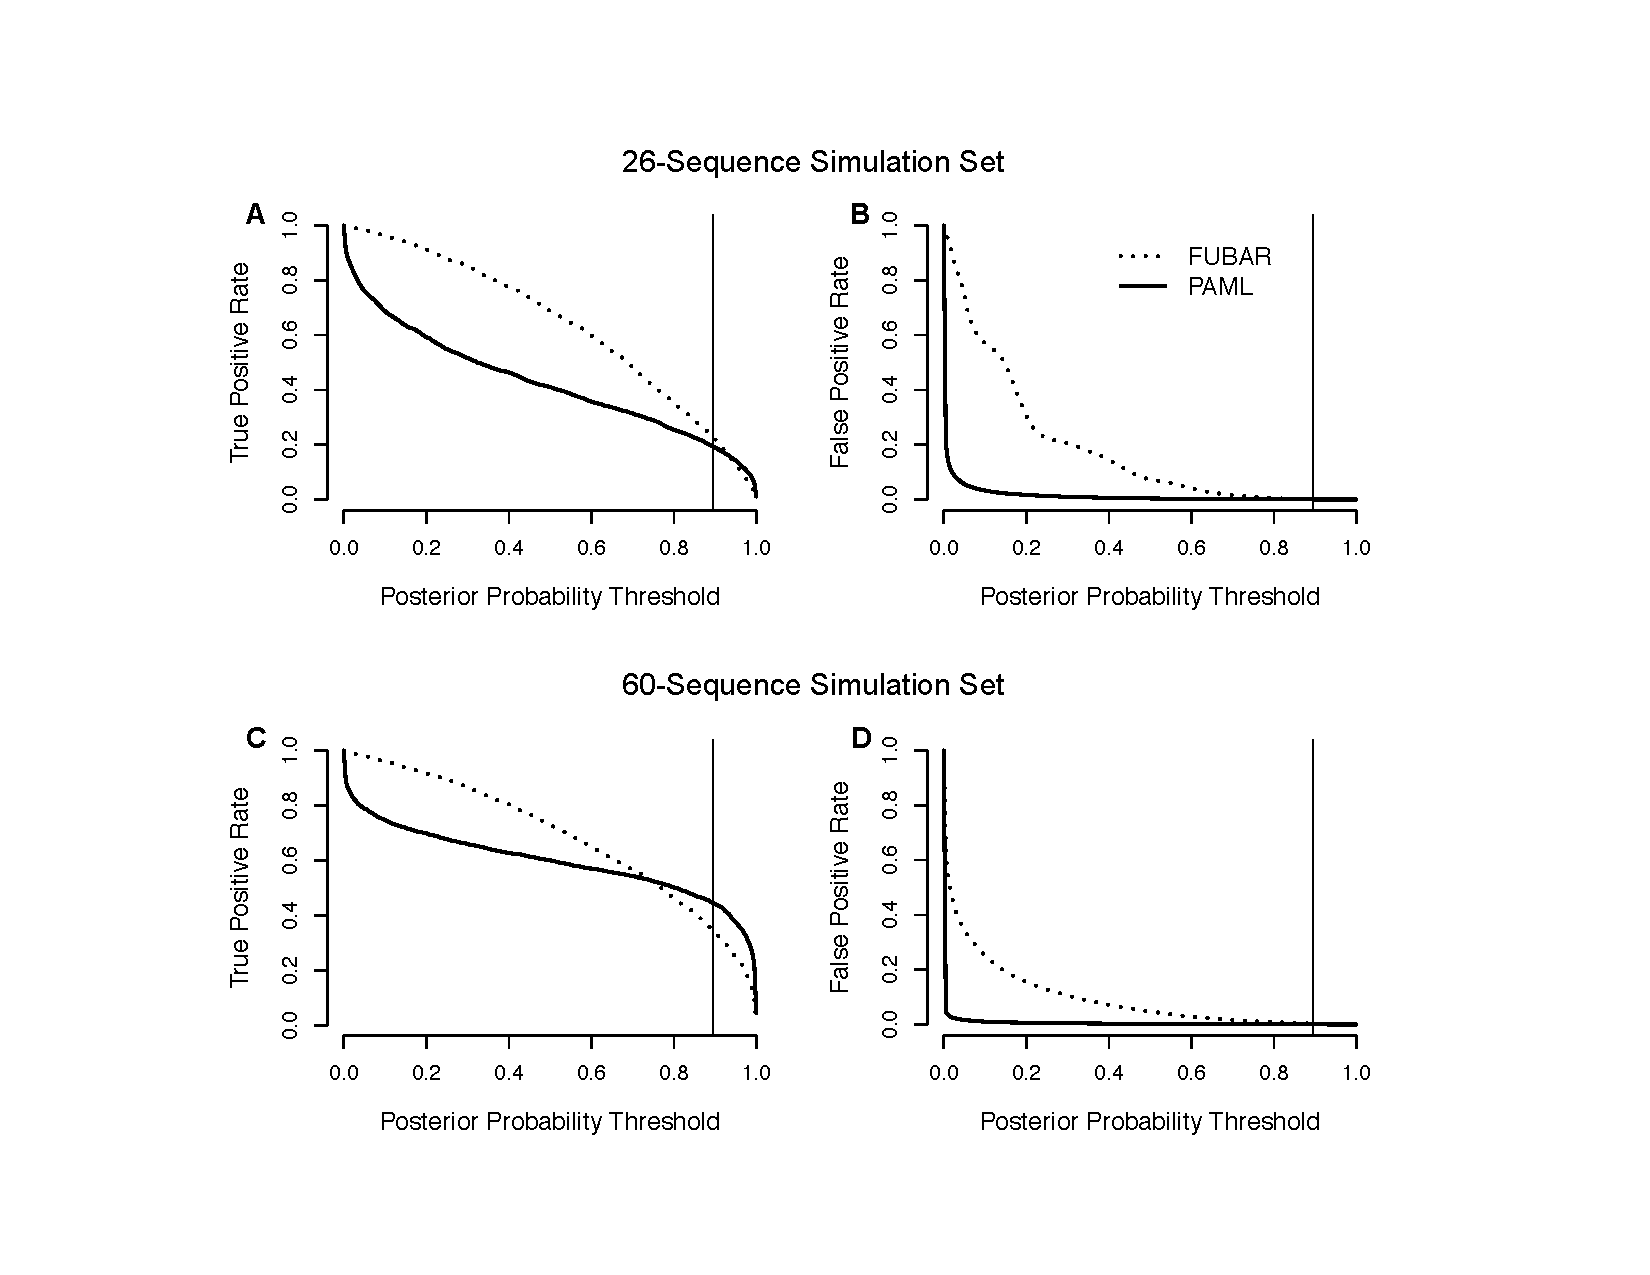
\includegraphics[width=7in]{Figures/tprfpr.pdf}}
\caption{True and false positive rates recovered from Fubar and Paml analysis with unfiltered alignments, averaged across the 26-sequence and the 60-sequence simulation sets, against the posterior probability threshold used to call sites as positively selected. A) TPR, 26-sequence set. B) FPR, 26-sequence set. C) TPR, 60-sequence set. D) FPR, 60-sequence set.  As the number of sequences increased, Paml's TPR improved at lower posterior probabilities, while its FPR remained remarkably low across all posterior probabilities for both simulation sets. While Fubar's performance did improve with the inclusion of more sequences, its overall TPR behavior did not change as dramatically as did Paml's.}
\end{figure*}



\begin{figure*}[H]
\centerline{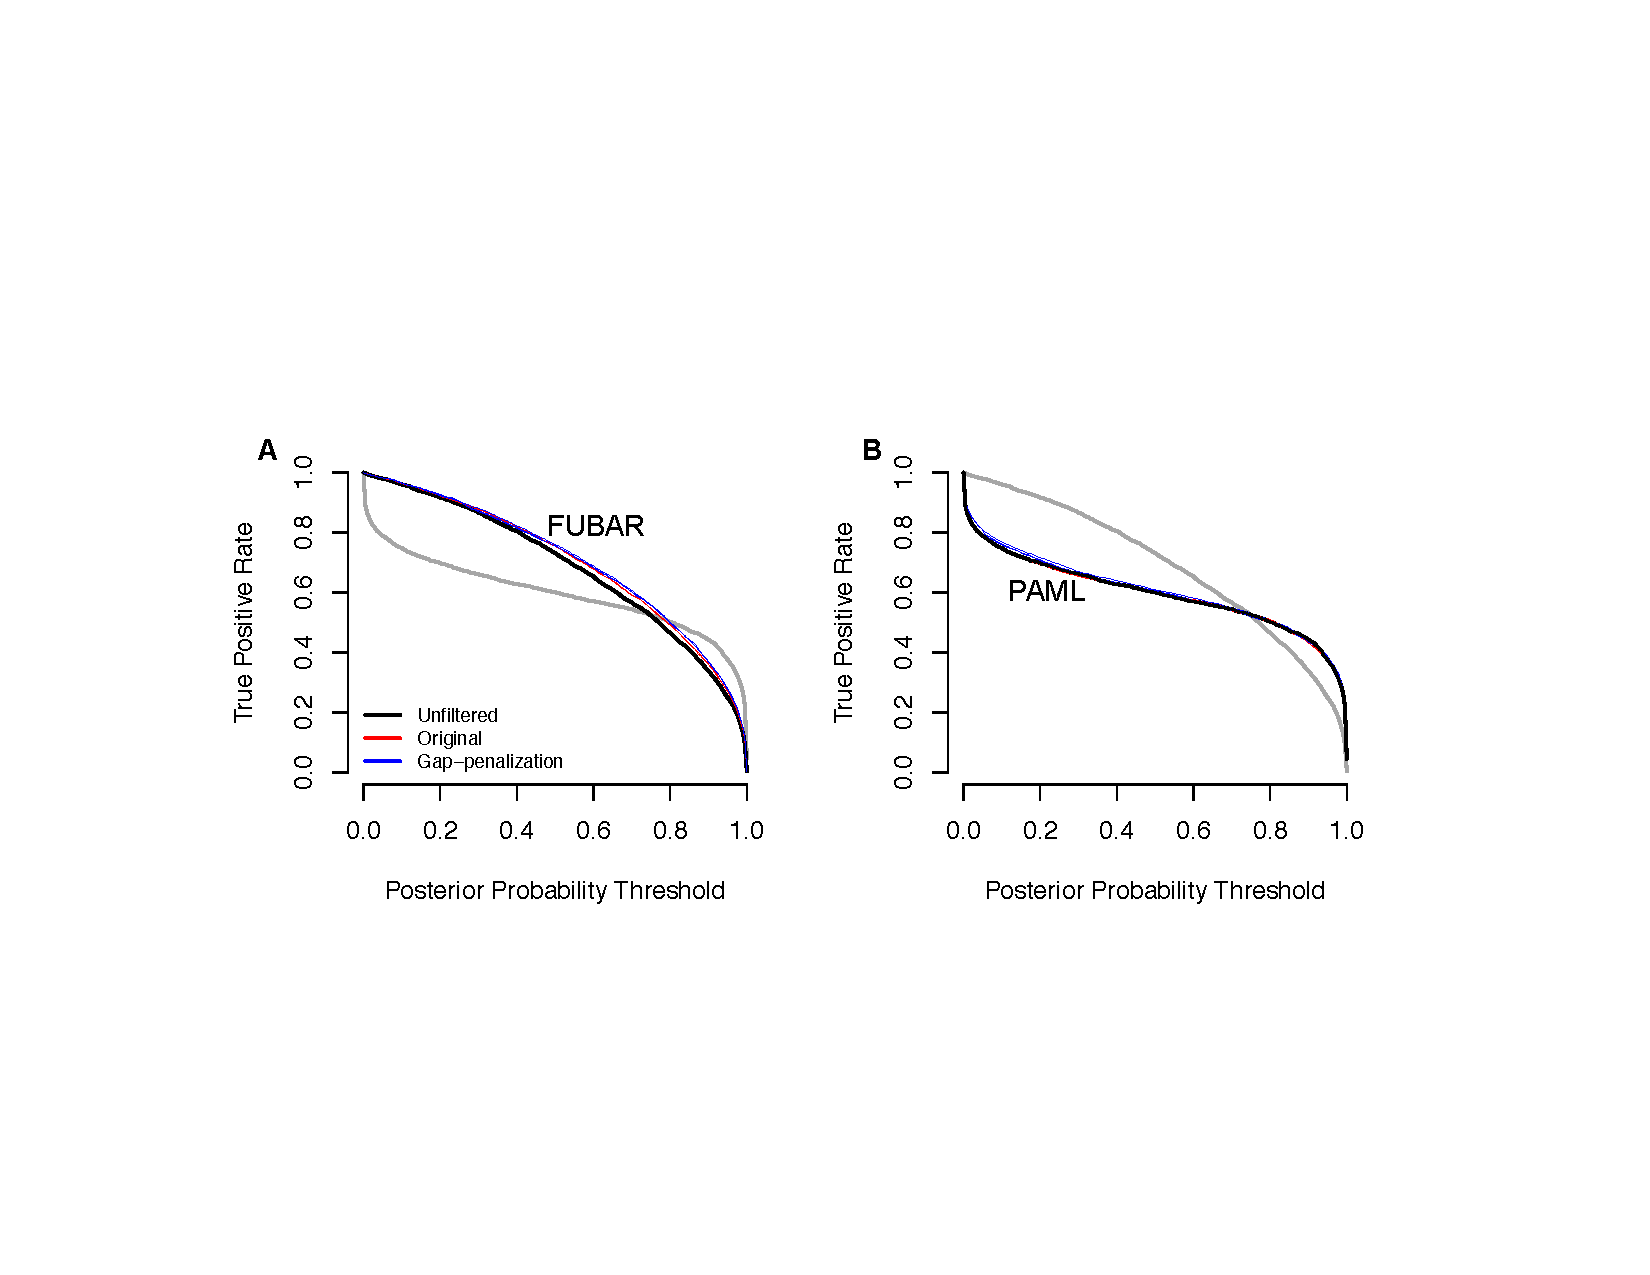
\includegraphics[width=7in]{Figures/fulltpr.pdf}}
\caption{\label{fulltpr} True positive rate against posterior probability threshold for calling positively selected sites, averaged across the 60-sequence simulation set. A) Fubar in color with Paml results shown in grey. B) Paml in color with Fubar results shown in grey. Filtered alignments behave similarly to unfiltered alignments across all posterior probabilities.}
\end{figure*}



\begin{table}[H]
\caption {\label{tab:penalmodel} Comparison of gap-penalization vs original normalization schemes on the true positive rate of positive-selection inference.}
\begin{tabular}{l l l l l l}
\hline\noalign{\smallskip}
\multicolumn{1}{c}{Simulation Set} & \multicolumn{1}{c}{Method} & \multicolumn{1}{c}{Guidance} & \multicolumn{1}{c}{BMweights} & \multicolumn{1}{c}{PDweights} \\
\noalign{\smallskip}\hline\noalign{\smallskip}
11 taxa  & Fubar & 0.001 (0.98\%) & $-1.76\times10^{-5}$ (-0.002\%) & 0.001 (0.95\%)\\
              & Paml & $-2.68\times10^{-4}$ (-0.31\%) & $2.57\times10^{-5}$ (0.03\%) & -0.001 (-1.50\%)\\
\hline
26 taxa   & Fubar & 0.0032 (1.38\%) & 0.00040 (1.75\%) & 0.0018 (0.77\%)\\
              & Paml & \textbf{0.006}$^{\ast}$ (3.02\%) & \textbf{0.007}$^{\ast\ast}$ (3.32\%) & 0.006$^{\ast}$ (2.89\%) \\
\hline
60 taxa  & Fubar & \textbf{0.010}$^{\ast}$ (2.67\%) & \textbf{0.012}$^{\ast\ast}$ (3.30\%)  & 0.005  (1.29\%)\\
              & Paml & -0.002 (-0.46\%) & 0.010 (2.23\%) & 0.008 (1.84\%) \\
\hline
158 taxa & Fubar & 0.003 (0.79\%) & 0.002 (0.48\%) & 0.001 (0.28\%)\\
\hline
\end{tabular}
\newline
\textsc{note.}--- Significance levels: $^{\ast\ast} P < 0.01$; $^{\ast} P < 0.05$. Each column displays the magnitude of TPR difference between normalization schemes, represented as gap-penalization minus original, for each algorithm, respectively. Percentage changes from the original normalization scheme are shown in parentheses. All significance levels were corrected for multiple comparisons with the single-step method.
\end{table}


\begin{table}
\caption {\label{tab:casemodel} Effect of alignment filtering on the true positive rate of positive-selection inference.}
\begin{tabular}{c c c l l l}
\hline\noalign{\smallskip}
& & & \multicolumn{3}{c}{Filtered TPR} \\
\cline{4-6}\noalign{\smallskip}
Simulation Set & Method & Unfiltered TPR & \multicolumn{1}{c}{GuidanceP} & \multicolumn{1}{c}{BMweightsP} & \multicolumn{1}{c}{PDweightsP} \\ 
\hline\noalign{\smallskip}
11 taxa  & Fubar & 0.108 & 0.109  (1.04\%)   & 0.110  (1.86\%)  & 0.110  (1.37\%)        \\
              & Paml &  0.087 & 0.088  (0.49\%) &  0.088  (0.83\%)   & 0.088  (0.79\%)        \\
\hline
26 taxa   & Fubar &  0.229 & 0.232 (1.54\%)  & 0.233 (1.83\%) & 0.233 (1.91\%)         \\
              & Paml & 0.194 & \textbf{0.204} (4.87\%)$^{\ast}$ & \textbf{0.203} (4.56\%)$^{\ast}$ & \textbf{0.203} (4.58\%)$^{\ast}$   \\
\hline
60 taxa  & Fubar & 0.345 & \textbf{0.379} (9.92\%)$^{\ast\ast}$ & \textbf{0.377} (9.31\%)$^{\ast\ast}$ & \textbf{0.375} (8.75\%)$^{\ast\ast}$  \\
              & Paml & 0.447 & 0.447 (0.19\%) & 0.440 (-1.43\%) & 0.445 (-0.30\%) \\
\hline
158 taxa & Fubar & 0.374 & \textbf{0.388} (3.89\%)$^{\ast\ast}$ & \textbf{0.387} (3.68\%)$^{\ast\ast}$ & \textbf{0.387} (3.47\%)$^{\ast\ast}$  \\
\hline
\end{tabular}
\newline
\textsc{note.}--- Significance levels: $^{\ast\ast} P < 1\times10^{-5}$; $^{\ast} P < 1\times10^{-4}$. \textit{Unfiltered TPR}: average true positive rate (TPR) for unfiltered alignments; \textit{Filtered TPR}: average true positive rate (TPR) for alignments filtered with each respective algorithm, with percent change from unfiltered alignment shown in parentheses. All significance levels are relative to the given simulation set's unfiltered alignment. We detected no significant TPR differences among filters tested within sequence simulation sets. All significance levels were corrected for multiple comparisons with the single-step method.
\end{table}



\bibliographystyle{MBE}
\bibliography{citations}	

\end{document}